\documentclass[a4paper]{article}
%\usepackage{fourier-otf}
\usepackage[utf8]{inputenc}
\usepackage{graphicx}
\usepackage{algorithm}
\usepackage{algpseudocode}
\usepackage{float}
\usepackage{lipsum}
\usepackage{scrextend}
\usepackage{biblatex}
\addbibresource{bibliography.bib}
\usepackage{listings}
\usepackage{amsmath}
\usepackage{amsfonts}
%\usepackage[square,sort,comma,numbers]{natbib}
\newtheorem{theorem}{Theorem}[section]
\usepackage{color}
\usepackage{makeidx}
\usepackage{titlepic}
\definecolor{mygreen}{rgb}{0,0.6,0}
\definecolor{mygray}{rgb}{0.5,0.5,0.5}
\definecolor{mymauve}{rgb}{0.58,0,0.82}
\lstset{ %
	backgroundcolor=\color{white},   % choose the background color
	basicstyle=\footnotesize,        % size of fonts used for the code
	breaklines=true,                 % automatic line breaking only at whitespace
	captionpos=b,                    % sets the caption-position to bottom
	commentstyle=\color{mygreen},    % comment style
	escapeinside={\%*}{*)},          % if you want to add LaTeX within your code
	keywordstyle=\color{blue},       % keyword style
	stringstyle=\color{mymauve},     % string literal style
}
\usepackage{hyperref}
\hypersetup{
  colorlinks   = true,    % Colours links instead of ugly boxes
  urlcolor     = black,    % Colour for external hyperlinks
  linkcolor    = black,    % Colour of internal links
  citecolor    = black      % Colour of citations
}
%\title{First chapter}

%\author{F.Bernardi}

%\protect\\ 

\newcommand{\myName}{Fabrizio Bernardi}
\newcommand{\myTitle}{Modeling and data analysis of the calcium activity in somatostatin interneurons from in vivo imaging on mice }
\newcommand{\myDegree}{Programme: \protect\\ \textit{Mathematical Engineering}}
\newcommand{\myCycle}{XXXI cycle}
\newcommand{\myDepartment}{Department of Mathematics}
\newcommand{\myUni}{Politecnico di Milano}
\newcommand{\myYear}{2022}
\newcommand{\myTime}{01 Jan \myYear}

\pdfbookmark{Cover}{cover}

\begin{document}
	
	
\section{Main tools for synchronization analysis}

In this chapter, the main tools for the analysis of synchronization between signals will be presented, with a focus on their mathematical definitions and their role in the application of \textit{Intebrain synchronization}.\\
After dealing with the problem of \textit{what} synchronization actually means in this context and which measures \textit{should not} be considered, several valid tools will be proposed:\textbf{ cross-correlation}, \textbf{peak-synchronization}, \textbf{angular similarity}, \textbf{$L^2$ error analysis}. Each one of these tools has a specific purpose and meaning, and they will all be considered in the analysis of this work, in order to give different shapes to the concept of synchronization and to try to study it under the largest possible perspective.\\
Finally, when observing the presence of correlation between two signals, a different (although strongly connected) question may arise: "which is the \textit{relationship} of such connection?", or, in other words, "is one signal dictating the behaviour of the other?". To answer such questions, a sophisticated tool will be object of study: the \textbf{Granger causality}.


\subsection{Understanding synchronization}

\begin{figure}[H]
	\begin{center}
		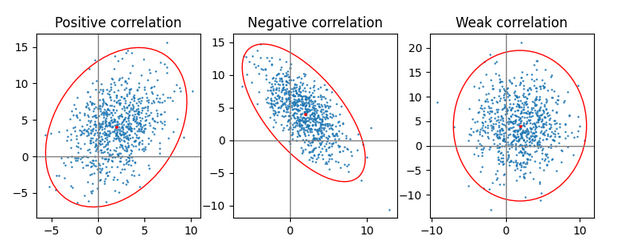
\includegraphics[scale=.75]{pearson.png} 
	\end{center} 
	\caption{\textit{Geometrical interpretation of the Pearson correlation: such coefficient gives a measure of how well the pairs obtained from the two samples distribute linearly along the diagonal of an ellipse covering the scatterplot. }}
	
\end{figure}

One of the main goals of this work will be to perform a data analysis on the Interbrain synchronization of neural signals, recorded in behavioural tasks. In order to do so, first one has to clarify the meaning of the term  \textit{synchronization}.\\
In a statistical sense, the synchronization between two time series can be seen as a measure of the \textbf{correlation} between them: the more two series are correlated, the more similar and connected they will be. This leads inevitably to the fact that, when talking about synchronization, the definition can't be unique, since the similarity between two series can be assumed in different ways, depending on the particular aspect of interest. \\
However, one first hint about what to look for or not can be found in the type of signal which is under analysis. In the case of this work, dealing with single neuron measurements of the intracellular concentration of $[Ca^{2+}]$ means dealing with \textit{strongly nonlinear and unstable signals}, which present sudden peaks and an often chaotic and difficult to predict behaviour .\\
For this reason, the measure of correlation which is probably the most famous and used, namely the \textbf{Pearson correlation}, is not suited to describe such signals. Given two random samples $ \textbf{x} = \{x_i\}_{i=1}^N$ and  $ \textbf{y} = \{y_i\}_{i=1}^N$, the Pearson correlation (PC) between them is defined as

$$ \rho(x,y) = \frac{Cov(x,y)}{\sigma_x \sigma_y} = \frac{\sum_{i=1}^{N}(x_i-\bar{x}) (y_i-\bar{y})} {\sum_{i=1}^{N}(x_i-\bar{x})^2 \sum_{i=1}^{N} (y_i-\bar{y})^2} $$

Where:
\begin{itemize}
	\item $ \bar{x} = \frac{1}{N}\sum_{i=1}^{N}x_i$ is the sample mean
	
	\item $Cov(x,y) = \frac{1}{N}\sum_{i=1}^{N}(x_i-\bar{x}) (y_i-\bar{y})$ is the sample covariance
	
	\item $\sigma_x = \sqrt{\frac{1}{N}\sum_{i=1}^{N}(x_i-\bar{x})^2}$ is the sample standard deviation
\end{itemize}

The PC measures the \textit{linear correlation} between two variables. This implies that this type of correlation should be used to inspect a linear relationship between two variables, which have a distribution close to the Gaussian one, and which presents uniform variance (i.e. reduced presence of outliers) [Applied multivariate statistics book by Johnson]. Unfortunately, with the type of data incoming from the neural recordings, all these hypoteses fail, and it follows that other correlation measures should be inspected instead.


\subsection{Cross-correlation}

When investigating the similarity between two signals depending on time, the first tool to be considered probably has to be the \textbf{cross-correlation}.\\
Formally, given two functions $ f = f(t)$ and $ g = g(t)$ , we define the cross-correlation between them as

\begin{equation}
[f(t) \star g(t)] (\tau) = \int_{-\infty}^{+\infty} f(\tau)g(t+\tau) dt 
\end{equation}


Given that the \textbf{convolution} between such functions is defined as 
\begin{equation}
[f(t) * g (t)](t) = \int_{-\infty}^{+\infty} f(t) g (t-\tau) d\tau
\end{equation}

it follows that
\begin{equation}
[f(t) \star g(t)](t) = [f(-t) * g (t)](t) 
\end{equation}

This means that the cross-correlation coincides with a convolution in which one function is considered backward in time. Moreover, in the common form of cross-correlation, as shown in (eq.1), the resulting quantity is not expressed as function of the time variable $t$, but as function of $\tau$, i.e. the \textit{lag} or \textit{delay} between the signals. The interpretation is straightforward: when, for a given value of the delay $\tau$, simultaneous peaks of the two signals are both present, the contribution of their product in the integral will be more relevant for the computed value of cross-correlation correspondent to  that specific lag.\\
As a consequence of this, once computing the cross-correlation between two time functions, one can identify its maximum value and retrieve the correspondent lag-value, from which it is possible to obtain an estimation of the delay between the two functions. To summarize, a cross-correlation analysis allows to:
\begin{enumerate}
	\item Compute the cross-correlation between the two signals as a function of the lag value  $\tau$
	
	\item Estimate the real delay between such signals, observing when the peak of cross-correlation happens
\end{enumerate}

When the cross-correlation is computed between the same function, it takes the name of \textbf{autocorrelation}. Confronting two identical signals, there will always be a peak of correlation (equal to $1$ using \textit{normalized} cross-correlation) correspondent to the lag $\tau = 0$. Moreover, the shape of the cross-correlation will be always symmetrical (see Figure).

\begin{figure}[H]
	\begin{center}
		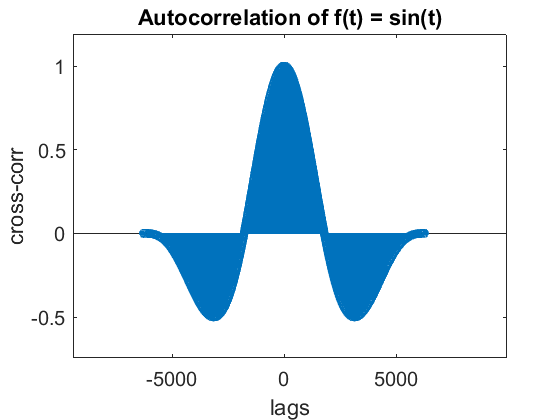
\includegraphics[scale=.75]{autocorr.png} 
	\end{center} 
	\caption{\textit{Aurocorrelation of the function $ f(t) = \sin(t) $}}
	
\end{figure}


While the autocorrelation represents an ideal case, when dealing with two different functions $f(t)$ and $g(t)$, the goodness of their cross-correlation will be given by the amount of shared properties to the case of autocorrelation; however, depending on the application in study, it could be normal to expect a peak value in correspondent to a nonzero value of the lag, as a representation of an actual physical delay.
\\

Given two time series $ \textbf{x} = \{x_i\}_{i=1}^N$ and  $\textbf{y} = \{y_i\}_{i=1}^N$, the discrete approximation of (eq.1) reads:


$$ [\textbf{x} \star \textbf{y}] (m) =  \sum_{n=1}^{N-1} x_n y_{n+m} \hspace{2cm} m_{min} < m < m_{max} $$

Where $m$ is the lag value, chosen in an appropriate interval.



\subsection{Peak-synchronization}

Cross-correlation is a general and widely used tool to quantify the similarity between two signals evolving in time, probably the most used and valid. With the following concept, the \textbf{peak-synchronization}, the focus of the analysis narrows to the specific type of signal characterizing this work: recording of intracellular calcium activity.\\
As it has been shown in Chapter 1, a typical recording of the activity of a single neuron is characterized by the presence of rapid and intense \textit{peaks}, which will define the neuron as \textit{active}. It follows that a way to intend synchronization between neurons could be related to the presence of \textit{close} or \textit{simultaneous} peaks observed at the same time. In other words, two signals (hence, neurons) will be synchronized, under the peak-synchronization point of view, if a \textit{pattern} of simultaneous firing emerges. 
\\

In order to quantify the peak-synchronization between two signals, the following steps have to be faced:

\begin{figure}[H]
	\begin{center}
		\hspace*{-3cm}
		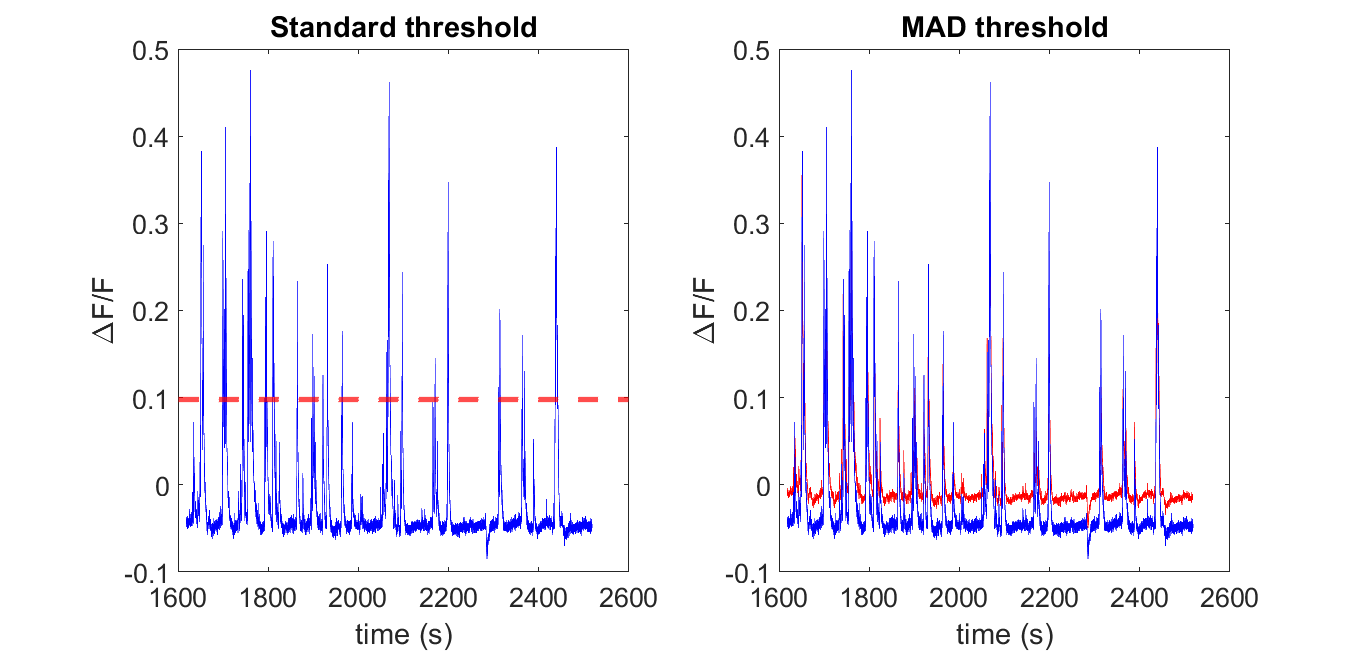
\includegraphics[scale=.50]{thresholds.png} 
	\end{center} 
	\caption{\textit{Example of a calcium signal (blu). The red curves are the thresholds built from the two algorithms: standard threshold (left) and MAD threshold (right)}}
	
\end{figure}

\begin{enumerate}
	
	\item Identify when a neuron is \textit{active}, i.e. when we are in presence of a peak
	
	\item Choose an appropriate time-interval in which two neurons firing simultaneously can be considered as synchronized
	
	\item Determine a way to quantify such correlation
	
\end{enumerate}



The way to solve all of these three steps is not unique, but it is strictly dependent on the current biological application under study and by the choice of appropriate algorithms and formulas for the activity detection and for the synchronization quantification. As for this work, the following considerations and choices have been made:




\begin{enumerate}
	
	\item Several algorithms are available or could be designed to detect, given a discrete time series, when a peak is happening. A straightforward idea is to establish a threshold for the activity, defining active all the points above it and non-active  all the ones below. Therefore, the output of such algorithm is of binary type ($1$ for activity, $0$ for non-activity).\\
	
	A naive way to create such threshold could be to consider a horizontal line, for example given by the equation $ y = \mu + 2\sigma $,	where $\mu$ and $\sigma$ are the mean and the standard deviation of the signal. In this way. All the values higher than this fixed quantity will be considered active and vice versa. This approach is good enough when dealing with "well-behaving" signals, presenting a baseline low activity alternated with huge peaks, however it seems to fail when dealing with more complex and noisy signals.\\
	\begin{algorithm}
		\caption{Standard threshold algorithm}\label{tresh}
		\begin{algorithmic}[1]
			
			
			\State Consider a horizontal threshold given by $ y = \mu + 2\sigma $
			
			\State Confront every point of the signal with their correspondent point of the threshold
			
			\State Every point above the threshold is labeled as $1$, all the points below as $0$
		\end{algorithmic}
	\end{algorithm}
	
	
	For this reason, a different algorithm can be considered as well [Inscopix manual]: the \textbf{MAD threshold} algorithm. The threshold established by this algorithm is not constant, but it "follows" the signal, in order to better capture its dynamism. 
	
	
	
	
	
	
	
	\begin{algorithm}
		\caption{MAD threshold algorithm}\label{mad}
		\begin{algorithmic}[1]
			
			
			\State Start from a baseline threshold given by $ MAD = median(X_i - median(X))$
			
			\State Identify the points where the slope changes from positive to negative (PN) and from negative to positive (NP)
			
			
			\State At every PN point, the threshold value is the MAD value plus the previous NP point's value
			
			\State The overall threshold is obtained from linear interpolation of the threshold points
			
			\State Every point above the threshold is labeled as $1$, all the points below as $0$
		\end{algorithmic}
	\end{algorithm}
	
	\item A typical time interval in which a firing happens usually strongly depends on the specific case. However, in general it is safe to say that the peak of a neuron usually last at least $250-500$ ms. Such value will define the reference time window. 
	
	\item Finally, once the binary vectors of activations are available, as well as a reference time window, to quantify the simultaneous synchronization, a common tool in literature is the \textbf{Peak-correlation index} [Cutts and Eglen], defined as 
	
	$$ i_{AB} = \frac{N_{AB} T}{2 N_A N_B dT} $$ 
	Here $T $ is the overall signal time window, $dT$ is the synchronization time window, $N_A$ is the number of peaks in signal A, $N_B $ is the number of peaks in signal B and finally $N_{AB} = \sum_{i=1}^{N_A} \sum_{j=1}^{N_B} I_{[-dT,dT]}(|a_i - b_j|) $ is the sum of simultaneous peaks along every synchronization window.
	
\end{enumerate}

The peak correlation index gives a representation of how well two signals (neurons) are peak-synchronized. However, it is necessary to notice that such measure is not normalized, meaning that the value of one index considered by itself has no real meaning, and this measure should be used only to compare different pairs.


\subsection{Angular distance and $L^2$ error}

\begin{figure}[H]
	\begin{center}
		\hspace*{-3.5cm}
		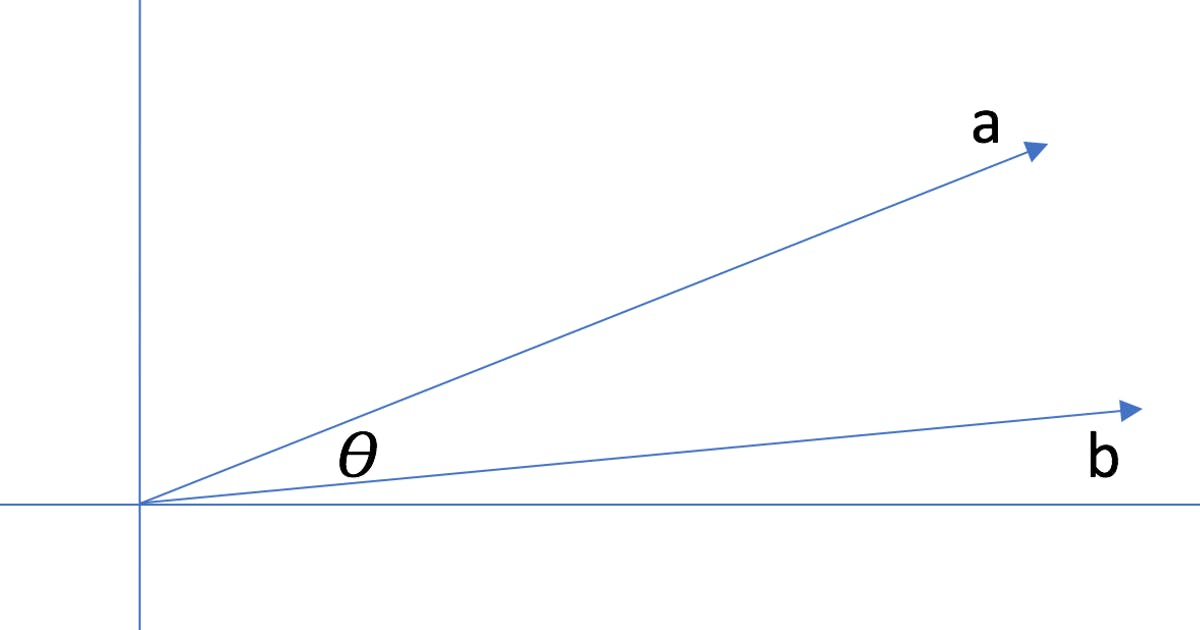
\includegraphics[scale=.20]{cos_sim.jpg} 
	\end{center} 
	\caption{\textit{Angle between two vectors in Euclidean space (2D case)}}
	
\end{figure}

After considering the two main tools for the synchronization analysis, cross-correlation and peak-synchronization, other concepts of correlation and similarity can be investigated as well. Here, two supplementary measures have been chosen: the \textbf{angular distance} and the \textbf{$L^2$ error}.
\\

The purpose of the angular distance analysis is to determine the similarity between two signals in a \textit{geometric sense}. The idea is indeed rather simple: project the signals on a Euclidean space and observe the angle between them. The two signals will be closer, and thus more similar, if the angle between them will be small.
A way to obtain the angle $\theta$ between two vectors is to compute first the \textbf{cosine similarity}

$$ Sim_C(\textbf{x},\textbf{y}) = \cos \theta =  \frac{\textbf{x} \cdot \textbf{y}}{||\textbf{x}||_E ||\textbf{y}||_E} $$

where $\textbf{x} \cdot \textbf{y}$ denotes the scalar product between $\textbf{x}$ and $\textbf{y}$ and $ ||\cdot||_E$ denotes the Euclidean norm.

Once computed the cosine of the angle, the angular distance can be retrieved as

$$ d_\theta (\textbf{x},\textbf{y}) = \frac{\arccos(Sim_C(\textbf{x},\textbf{y}))}{\pi} $$

Where the actual angle is divided by a reference $\pi$ angle.
\\
As for the $L^2$ error, between two continuous functions $f$ and $g$ defined on an interval $[t_1,t_2]$, the $L^2$ error between them is defined as 

$$ ||f-g||_2 = \int_{t_1}^{t_2}|f(t) - g(t)|^2 dt $$

When dealing with a discrete approximation, it actually coincides with the \textbf{mean squared error (MSE)}

$$ MSE(\textbf{x},\textbf{y}) = \frac{1}{N}\sum_{i=1}^{N}|x_i-y_i|^2 $$


The MSE analysis performs a point-by-point comparison of the two signals, penalizing quadratically the differences between the two. It follows that in order to have a realistic estimate of this error, it is necessary to confront well-aligned signals. For this purpose, a previous analysis of cross-correlation can be helpful, since, as described in section (2.2), such analysis can also identify the \textit{delay} between two time series, detected in correspondence to the cross-correlation peak. In conclusion, an alignment based on such value of lag between the two time signals should be performed before this $L^2$ error analysis.



\subsection{Granger causality}


\begin{figure}[H]
	\begin{center}
		\hspace*{-1cm}
		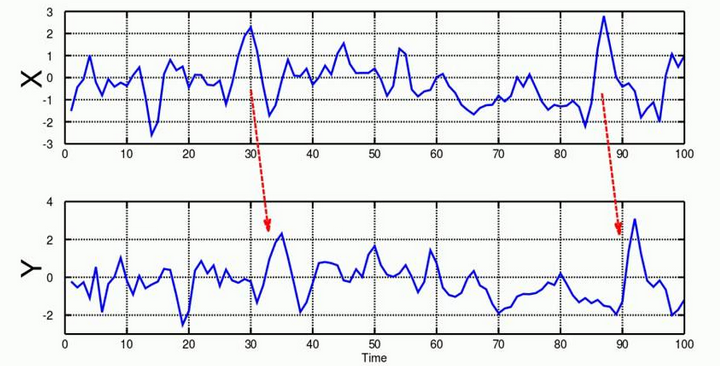
\includegraphics[scale=.60]{GC.png} 
	\end{center} 
	\caption{\textit{Example of signal X Granger-predicting signal Y }}
	
\end{figure}

As already mentioned in section (1.5), observing a correlation between two time series 
is not enough to establish a \textit{relationship} between them. Indeed, a parallel issue to the synchronization between signals is the presence of a \textit{cause-effect} mechanism underlying it all. If such relationship is found, besides observing a synchronization, one can find as well which signal (and, in this case, mouse) is responsible for causing the opponent's one.\\
In situations like the EEG experiment in [Novembre et al.] discussed in the previous chapter, such relationship had been investigated through a manipulation on an experimental level. In the case of the current work, once dealing with data already measured, a different and sophisticated approach is adopted, relying on straightforward statistical principles: the \textbf{Granger causality}.\\
The Granger causality (\textbf{G-causality}) is a method aimed to identify causal relationship between time series data. The adjective "casual" is mainly due to historical reasons, since many debates about its correctness are still ongoing, and it would be probably more precise to refer to it as "Granger \textit{prediction}".
\\

Given two time series $ \textbf{x} = \{x_i\}_{i=1}^N$ and  $\textbf{y} = \{y_i\}_{i=1}^N$, the main ideas of the G-causality method rely on the following scheme:

\begin{enumerate}
	
	\item Creation of a \textbf{vector autoregression model (VAR)} of order $p$, integer to be determined, for one of the two time series, considering its previous values
	
	\begin{equation}
	\hat{x}_t = a_0 + a_1 x_{t-1} + a_2 x_{t-2} + \dots + a_p x_{t-p}
	\end{equation}
	
	
	\item Creation of a second model, in which the values of the second series are added  to the previous model 
	\begin{equation}
	\hat{x}_t = a_0 + a_1 x_{t-1} + a_2 x_{t-2} + \dots + a_p x_{t-p} + b_1 y_{t-1} + \dots + b_p y_{t-p}
	\end{equation}
	
	
	\item Comparison of the two models: if model 2 is more significant (in a way which will be clarified in the following) than model 1, then signal $\textbf{y}$ \textit{Granger-predicts} signal \textbf{x} 
	
\end{enumerate}

More formally [Barnett-Seth], given two stochastic processes $ \textbf{X} = {X}_{i=1}^N $ and $ \textbf{Y} = {Y}_{i=1}^N $, process Y \textit{does not} G-cause process X if X, conditional its past, is independent by the past of Y. A vector autoregressive model for a process $U$ takes the form

\begin{equation}
\textbf{U}_t = \sum_{k=1}^{p} A_k \textbf{U}_{t-k} + \varepsilon_t 
\end{equation}



Where $p$ is the \textbf{order} of the model, $\{ A_k\}$ are the \textbf{regression coefficients} and $\varepsilon$ the \textbf{residuals}, assumed normally and independently distributed. The \textbf{ residual covariance matrix} of the model is defined as $ \Sigma = Cov(\varepsilon_t) $ and it is assumed to be stationary. The process $U$ can then be identified both as $X$ and $Y$. Given a VAR model of the form (6), the \textbf{autocovariance sequence} $ \{\Gamma_k\} $ is defined as $ \Gamma_k = Cov(\textbf{U}_t,\textbf{U}_{t-k})$, and it is possible to relate this quantity to the autoregression coefficients $\{ A_k\}$ thanks to the \textbf{Yule-Walker} equations [Anderson,1971]

\begin{equation}
\Gamma_k = \sum_{i=1}^{p} A_i \Gamma_{k-i} + \delta \Sigma \hspace{1 cm }  \delta \in \mathbb{R}
\end{equation}\\

Standard VAR theory [Hamilton-Lutkephol], requires, for the validity of this analysis, the condition $ \sum_{k=1}^{N}||A_k||^2 < \infty $. Moreover, defining the \textbf{characteristic polynomial} as 
$$ \phi_A(z)= \left| I - \sum_{k=1}^{p} A_k z^k \right| $$
it must be that the \textbf{spectral radius} $\rho(A) := \max_{\phi_A(z)=0}|z|^{-1}$ is strictly less than $1$, as a \textit{stability} condition.
\\

Considering now a process in which $ \textbf{U}_t = \begin{bmatrix} \textbf{X}_t  \\  \textbf{Y}_t \end{bmatrix} $, its VAR formulation reads

\begin{equation}
\textbf{U}_t = \sum_{k=1}^{p} \begin{bmatrix} A_{xx,k}  &  A_{xy,k} \\  A_{yx,k}  & A_{yy,k} \end{bmatrix} \textbf{U}_{t-k} + \begin{bmatrix} \varepsilon_{x,t}  \\  \varepsilon_{y,t} \end{bmatrix}
\end{equation}


And its residual covariance is $ \Sigma = Cov\left(\begin{bmatrix} \varepsilon_{x,t}  \\  \varepsilon_{y,t} \end{bmatrix}\right) = \begin{bmatrix} \Sigma_{xx}  &  \Sigma_{xy} \\  \Sigma_{yx}  & \Sigma_{yy} \end{bmatrix} $.\\
This augmented formulation contains both the regression models for process $X$ and $Y$. For example, its first component reads

\begin{equation}
\textbf{X}_t = \sum_{k=1}^{p} A_{xx,k} \textbf{X}_{t-k} + \sum_{k=1}^{p} A_{xy,k}  \textbf{Y}_{t-k} + \varepsilon_{x,t}
\end{equation}

If the process $Y$ does not G-cause the process $X$, it will follow that the coefficients $\{A_{xy,k}\}_{k=1}^p $ will be all null, and the model will take a form

\begin{equation}
\textbf{X}_t = \sum_{k=1}^{p} A'_{xx,k} \textbf{X}_{t-k} + \varepsilon'_{x,t}
\end{equation}

Therefore, a statistic test checking on the null hypothesis \{$ H_0:  Y \hspace{0.2cm} \text{does not G-predicts} \hspace{0.2 cm} X $\} has the form

\begin{equation}
H_0: A_{xy,1} = A_{xy,2} = \cdots = A_{xy,p} = 0
\end{equation}


If  $\Sigma'_{xx} = Cov(\varepsilon'_{x,t}) $ is the residual covariance matrix of model (10), standard theory [Edwards, 1992] suggests the use of the \textbf{(log-)likelihood statistics} to obtain a \textit{maximum-likelihood} estimator of the G-causality between $Y$ and $X$ (here referred as $ \mathcal{F}_{Y \rightarrow X} $):

\begin{equation}
\mathcal{F}_{Y \rightarrow X}  = \ln \frac{|\Sigma'_{xx}|}{|\Sigma_{xx}|}
\end{equation}


Since the determinant of a covariance matrix (i.e. the \textit{generalized variance}) quantifies the \textit{prediction error} of its regression model, the interpretation of (11) is that the G-causality statistics  $ \mathcal{F}_{Y \rightarrow X} $ is a measure of how much the prediction error is reduced when the process $Y$ is included in the regression model as well. Clearly, this same procedure applies as well for the statistics  $ \mathcal{F}_{X \rightarrow Y} $, in which the directionality of the relationship is inverted. It can be proven [Wilks \& Wald] that, under the null hypothesis, $ (N-p)\mathcal{F}_{Y \rightarrow X} \sim \chi^2(d)$, where $ d = pN^2$.
\\
To summarize, the typical workflow for G-causality estimation, consists in the following steps:

\begin{enumerate}
	\item Estimation of the model order $p$ via appropriate criterion (such as AIC and BIC)
	
	\item Estimation of the autocovariance sequence $\Gamma_k$ and the VAR coefficients $(A_k, \Sigma)$ through the Yule-Walker equations (7), both for reduced and augmented models. Check for the satisfaction of the validity hypotheses
	
	\item Computation of the G-statistics $ \mathcal{F}_{Y \rightarrow X} $ and $ \mathcal{F}_{X \rightarrow Y} $ through (12)
	
	\item Testing of the significance of the statistical tests against the null hypotesis, computing the p-values of the two tests 
	
\end{enumerate}




\end{document}


